\begin{adjustbox}{width=\textwidth}
	\begin{tikzpicture}[every node/.style={inner sep=0,outer sep=0}]
	
		\node [anchor=north east] (imgGlatt) at (-0.03\textwidth,0) {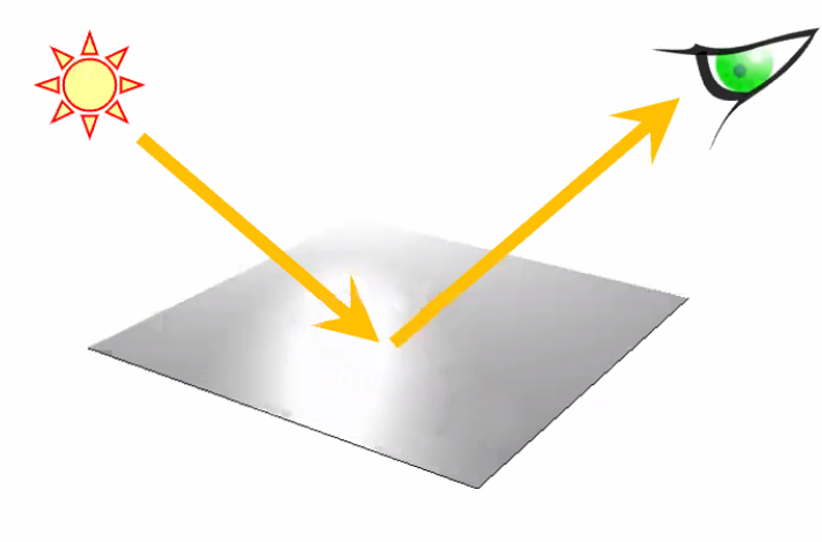
\includegraphics[width=.47\textwidth]{02_grundlagenZurDeflektometrie/spiegelndeOberflaechen/figures/spiegelnd}};
		\node [below=0.2cm of imgGlatt, align=center] {Spiegelnde Oberfläche mit glatter \\ Oberflächenbeschaffenheit};
		\node [anchor=north west] (imgRau) at (0.03\textwidth,0) {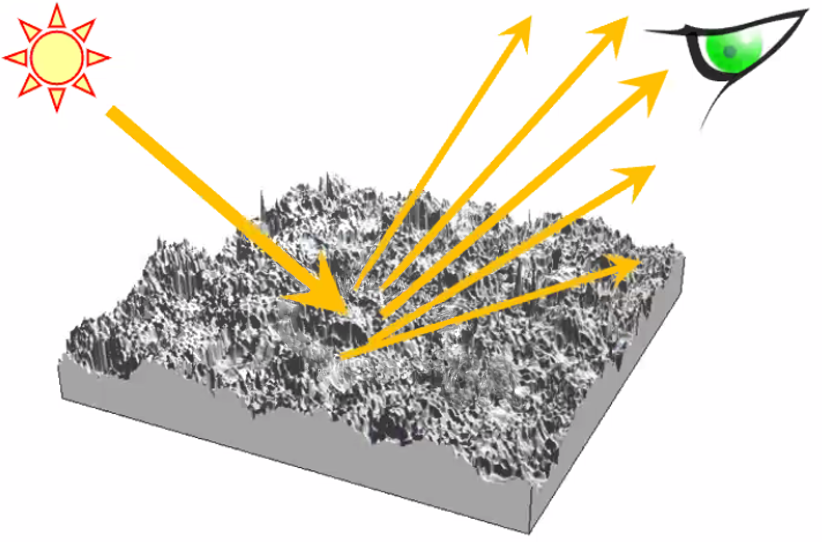
\includegraphics[width=.47\textwidth]{02_grundlagenZurDeflektometrie/spiegelndeOberflaechen/figures/rau}};
		\node [below=0.2cm of imgRau, align=center] {Matte Oberfläche mit rauer \\ Oberflächenbeschaffenheit};
		
	\end{tikzpicture}
\end{adjustbox}
\caption[Spiegelnde und matte Oberflächen]{Spiegelnde bzw. glatte und matte bzw. raue Oberflächen in ihrer mikroskopischer Oberflächenbeschaffenheit. \cite{jenaerOK}}